% !Mode:: "TeX:UTF-8"
%% 请使用 XeLaTeX 编译本文.制作者:中南大学,电气1705陈宝轩,2020.1.16
% \documentclass{WHUBachelor}% 选项 forprint: 交付打印时添加, 避免彩色链接字迹打印偏淡. 即使用下一行:
 \documentclass[forprint]{CSUBachelor}
\usepackage{listings}				%对代码进行抄录环境的宏包
\usepackage{setspace}				%行间距
\usepackage{float}

\begin{document}

\title{中南大学本科毕业设计~\LaTeX~模板}
\Etitle{A \LaTeX~Thesis Template for Zhongnan University} % 英文题目
\author{陈宝轩}                            		% 作者名字
\Eauthor{CHEN Baoxuan}           		 %作者英文名
\Csupervisor{老师姓名\quad 教授}       	 %指导教师中文名、职称
\Esupervisor{Prof.cc}    				 %指导教师英文名、职称
\Cmajor{电气工程及其自动化}                 	 % 专业中文名
\Emajor{Electrical Engineering and Automation}% 专业英文名
\Cschoolname{自动化学院}         		 % 学院名
\Eschoolname{School of Automation} 		%学院英文名.
\Cclassname{电气1705班}      			%专业班级中文名

\date{20XX年6月}                    		% 日期, 要注意和英文日期一致!!
\Edate{May, 2020}                      	 % 英文封面日期

%-----------------------------------------------------------------------------
\pdfbookmark[0]{封面}{title}         % 封面页加到 pdf 书签
\maketitle
\frontmatter
\pagenumbering{Roman}              % 正文之前的页码用大写罗马字母编号.
%-----------------------------------------------------------------------------
% !Mode:: "TeX:UTF-8"

%自行填写: (1) 中文摘要及关键词 (2) 英文摘要及关键词

%------------------------------------------中文摘要----------------------------------------------------
\begin{cnabstract}

本文在武汉大学模板的基础上,主要介绍和讨论了中南大学本科毕业论文的~\LaTeX~模板.

指明了编译方法,讨论了一些\LaTeX{}的使用小技巧
\end{cnabstract}
\par
\vspace*{1em}	%空一行,再写关键词

%-------------------------------------- 关键词 ---------------------------------------------------
%注意: 每个关键词之间空一格汉字的长度,最后一个关键词后无标点符号
\cnkeywords{\LaTeX{} \phantom{哈}中南大学\phantom{哈}模板\phantom{哈}陈宝轩想睡觉}

%------------------------------英文摘要---------------------------------------

\begin{enabstract}
This thesis is a study on the theory of \dots.

\end{enabstract}
\par
\vspace*{2em}

%------------------------------- Key words ---------------------------------------
%%%%-- 注意: 每个关键词之间空两个英文字母的长度,最后一个关键词后无标点符号
 \enkeywords{\LaTeX{}\phantom{cc}CSU\phantom{cc}template\phantom{cc}sleepy}
    % 加入摘要
%-------------------------------把目录加入到书签---------------------------------%
\pdfbookmark[0]{目录}{toc}
\tableofcontents
\mainmatter
%----------------------------------------------正文-------------------------------------%
\chapter{绪论}
 \section{具体使用步骤}
 \begin{description}
  \item[Step 1]  进入 includefile 文件夹,  打开 frontmatter.tex, backmatter.tex 这两个文档,
        分别填写 (1) 中文摘要、英文摘要, (2) 致谢.

  \item[Step 2]  打开主文档 Bachelor--template.tex, 填写题目、作者等等信息, 书写正文.

  \item[Step 3]  使用 XeLaTeX 编译. 具体见 \ref{sec-compile} 节.
\end{description}

\section{编译的方法}\label{sec-compile}

默认使用 XeLaTeX 编译, 直接生成~pdf 文件.

\section{文档类型选择}
文档类型有 2 种情形:

\begin{table}[ht]\centering
\begin{tabular}{ll}
\hline
   \verb|\documentclass{WHUBachelor}|                     &  毕业论文 \\
   \verb|\documentclass[forprint]{WHUBachelor}|        &  毕业论文打印版 \\
\hline
\end{tabular}
\end{table}

\chapter{模板格式说明}

\section{文章结构}

模板文件的结构, 如下表所示:

 \begin{table}[ht]\centering
\begin{tabular}{r|r|l}
	\hline\hline
	\multicolumn{2}{l|}{Bachelor-template.tex }       & 主文档. 在其中填写正文.             \\ \hline
	                                & frontmatter.tex & 郑重声明、中英文摘要.               \\ \cline{2-3}
	\raisebox{1em}{includefile 文件夹} &  backmatter.tex & 致谢.                       \\ \hline
	\multicolumn{2}{l|}{figures 文件夹}                  & 存放图片文件.                   \\ \hline
	\multicolumn{2}{l|}{CSUBachelor.cls }             & 定义文档格式的 class file. 不可删除. \\ \hline\hline
\end{tabular}
\end{table}

\section{更新记录}

2020年 01 月 16日更新: 进一步进行修改并完善(陈宝轩)

2020年 01 月 13日更新: 以武汉大学的模板为原型,根据中南大学的毕业设计论文模板要求,进行了修改,删除了一些不必要的内容,并增加了一些新的格式(陈宝轩)

\section{字体调节}

\begin{tabular}{ll}
	\verb|\songti|   & {\songti 宋体}   \\
	\verb|\heiti|    & {\heiti 黑体}    \\
	\verb|\fangsong| & {\fangsong 仿宋} \\
	\verb|\kaishu|   & {\kaishu 楷书}
\end{tabular}


\section{字号调节}
字号命令: \verb|\xiaosi| \index{zihao}

即为小四号字体

\section{标点符号的问题}

建议使用半角的标点符号, 后边再键入一个空格. 特别是在英文书写中要注意此问题!

双引号是由两个左单引号、两个右单引号构成的: \verb|``  ''|. 左单引号在键盘上数字~1 的左边.

但是, 无论您偏向于全角或半角, 强烈建议您使用实心的句号, 只要您书写的是自然科学的文章.
原因可能是因为, 比如使用全角句号的句子结尾处的``$x$。''容易误为数学式~$x_0$(\verb|$x_0$|)吧.


\section{引用的问题}


\subsection{参考文献的引用}

参考文献的引用, 用命令~\verb|\cite{ }|. 大括号内要填入的字串, 是自命名的文献条目名.

比如, 通常我们会说:

 {\kaishu
关于此问题, 请参见文献 \cite{r2}. 作者某某还提到了某某概念\upcite{r1}.}


上文使用的源文件为:

 {\kaishu
关于此问题, 请参见文献~\verb|\cite{r2}|. 作者某某还提到了某某概念~\verb|\upcite{r1}|.
}

其中~\verb|\upcite| 是自定义命令, 使文献引用呈现为\CJKunderdot{上标形式}.

({\heiti 注意:} {\kaishu 这里文献的引用, 有时需要以上标形式出现, 有时需要作为正文文字出现, 为什么?})

另外, 要得到形如~\cite{r1,r3,r4,r5} 的参考文献连续引用, 需要用到 cite 宏包(模板已经加入),
在正文中使用~\verb|\cite{r1,r3,r4,r5}| 的引用形式即可.
或者, 连续引用的上标形式: 使用~\verb|\upcite{r1,r2,r3}|, 得到\upcite{r1,r2,r3}.

\subsection{定理和公式的引用}

\begin{theorem}[谁发现的]\label{th-abcd}
最大的正整数是~$1$.
\end{theorem}

\begin{proof}
要找到这个最大的正整数, 我们设最大的正整数为~$x$, 则~$x \geqslant 1$, 两边同时乘以~$x$, 得到
\begin{equation}\label{eq-abc}
x^2 \geqslant x.
\end{equation}
而~$x$ 是最大的正整数, 由~\eqref{eq-abc} 式得到
\[
x^2 = x.
\]
所以
\begin{equation*}
x = 1.
\end{equation*}
\end{proof}

定理~\ref{th-abcd} 是一个重大的发现.
%------------------------------------定义等环境的举例 ----------------------------------------
\begin{definition}[整数]
 正整数(例如 1, 2, 3)、负整数(例如 ${−1}$, $−2$, $−3$)与零(0)合起来统称为{\heiti 整数}.
\end{definition}

\begin{remark}
  整数集合在数学上通常表示为 $\mathbf{Z}$ 或 $\mathbb{Z}$, 该记号源于德语单词 Zahlen(意为``数'')的首字母.
\end{remark}

\begin{proposition}
任意两个整数相加、相减、相乘的结果, 仍然是整数.
\end{proposition}

\begin{example}
  $1+2=3$.
\end{example}

\begin{corollary}
   在整数集合内, 相加、相减、相乘运算是封闭的.
\end{corollary}

\section{图形与表格}

支持对png, pdf, jpg 等等常见图形格式.

\begin{figure}[H]
\centering
%\setlength{\abovecaptionskip}{0pt}\setlength{\belowcaptionskip}{10pt}
\setlength{\abovecaptionskip}{2pt}\setlength{\belowcaptionskip}{10pt}	
%将图片标题紧靠图片		这个管用,表格的不管用
  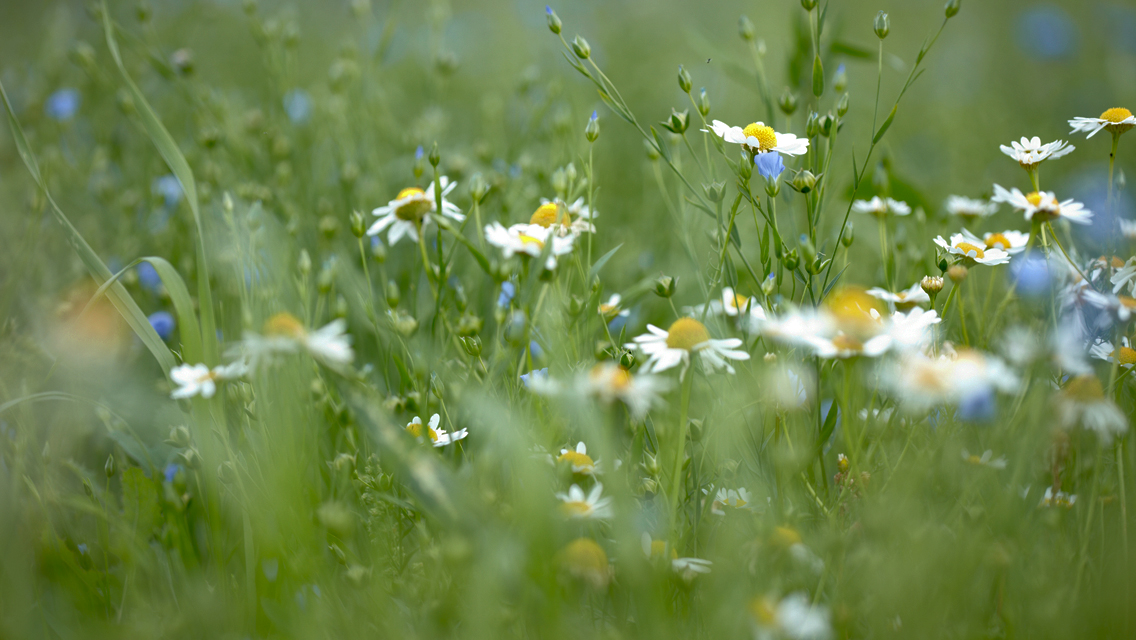
\includegraphics[width=\textwidth]{Daisy.jpg}
  \caption{\heiti\zihao{5}一个彩色 jpg 图片的例子}
  \label{fig:1}
\end{figure}

表格问题, 建议使用``三线表'', 如表 \ref{tab:1}.

\begin{table}[H]
%\begin{table}[ht]
\centering
\caption{\heiti\zihao{5}一般三线表}
\label{tab:1}
\vspace*{-10pt}	%表格向上10pt,将表格紧靠表头,我只想到了这一个办法。。。
    \begin{tabular}{c c c c c c c c c c c}
    \hline
    123 & 4  & 5  & 123 & 4 & 5123 & 4 & 5 & 123 & 4 & 5\\
    \hline
    67 & 890 & 13 & 123 & 4 & 5123 & 4 & 5 & 123 & 4 & 5\\
    67 & 890 & 13 & 123 & 4 & 5123 & 4 & 5 & 123 & 4 & 5\\
    67 & 890 & 13 & 123 & 4 & 5123 & 4 & 5 & 123 & 4 & 5\\
    \hline
    \end{tabular}
\end{table}


%--------------------------------------------其他事项--------------------------------------------------

\chapter{其他事项}
由于是采用武汉大学的模板为原型,因此他们的广告我就不删除了。

若在使用次中南大学毕业设计论文模板的过程中遇到任何问题或有更好的改进想法,欢迎联系作者{\bf\uline{QQ:1431702599}}进行交流。

\vspace{1em}
以下为武汉大学他们的广告,此处原封不动地保留,感谢武汉大学的模板制作者们对我在\LaTeX{}学习上起到的帮助:
\begin{itemize}
    \item 插图\index{插图}的制作, 建议用 pgf, 也叫 tikz.
          pgf 的长处是源文件直接植入~\TeX~文档, 管理起来非常方便.
    这里有我写的一个关于初次使用~pgf~的帖子:\\    \url{http://bbs.ctex.org/forum.php?mod=viewthread&tid=30480}.
    \item 生成参考文献, 建议使用~BibTeX.\index{BibTeX} 这里有我写的一个文档: \\
    \url{http://bbs.ctex.org/forum.php?mod=viewthread&tid=26056}.

          {\kaishu 使用 BibTeX{} 做参考文献时,
      借助 EndNote 或者 NoteExpress, 可以非常漂亮简单地解决 bib 文件的录入问题.
      NoteExpress 在校图书馆网站有正版软件提供下载.
      当然 EndNote 本身就是 Thomson Corporation 推出的(和 SCI 搜索引擎是同一家公司),
      和多个重要文献搜索引擎有良好的功能配合.

      Google 学术搜索也提供了文献的 bib 格式.
      录入参考文献时, 偶尔用一用 Google 学术搜索, 还可以核查或减少录入的错误, 并减少录入的工作量.}

    \item 幻灯片\index{幻灯片}的制作, 建议使用~Beamer. 这里有我写的一个模板, 谨供参考:\\
    \url{http://bbs.ctex.org/forum.php?mod=viewthread&tid=27695}.
    
     \item 武汉大学模板下载更新地址:
  \url{http://aff.whu.edu.cn/huangzh/}
\end{itemize}


%--------------------------------------------- 结束语 -------------------------------------------
% !Mode:: "TeX:UTF-8"
%-----------------------------结束语(或致谢)---------------------------------

\acknowledgement
\addcontentsline{toc}{chapter}{结束语(或致谢)}

(结束语或致谢内容)











 		%致谢

%--------------------------------------------- 参考文献 -------------------------------------------
\cleardoublepage\phantomsection
\addcontentsline{toc}{chapter}{参考文献}
\wuhao\kaishu
\begin{thebibliography}{00}

  \bibitem{r1} 作者. 文章题目 [J].  期刊名, 出版年份,卷号(期数): 起止页码.

  \bibitem{r2} 作者. 书名 [M]. 版次. 出版地:出版单位,出版年份:起止页码.

  \bibitem{r3} 邓建松等, 《\LaTeXe~科技排版指南》, 科学出版社.

  \bibitem{r4} 吴凌云, 《CTeX~FAQ (常见问题集)》, \textit{Version~0.4}, June 21, 2004.

  \bibitem{r5} Herbert Vo\ss, Mathmode, \url{http://www.tex.ac.uk/ctan/info/math/voss/mathmode/Mathmode.pdf}.

\end{thebibliography}

%----------------------------------- 附录-----------------------------------
\appendix

\chapter{测试}

\section{第一个测试}
测试公式编号
\begin{equation}
1+1=2.
\end{equation}

表格编号测试

\begin{table}[h]
  \centering
  \caption{测试表格}
  \begin{tabular}{*{20}c}
     \hline
     % after \\: \hline or \cline{col1-col2} \cline{col3-col4} ...
     11 & 13  & 13  & 13  & 13 \\
     12 & 14  & 13  & 13  & 13 \\
     \hline
   \end{tabular}
\end{table}


\chapter{源代码}

\section{第一部分代码}

%设置·为转义字符,这样才可以显示汉语
\lstset{columns=flexable,numbers=left,numberstyle=\footnotesize,escapechar=`,xleftmargin=2em,xrightmargin=2em, aboveskip=0em}

\begin{spacing}{1}
\begin{lstlisting}[language=C]
/*hello.c*/
#include "sys.h"
int main(void)
{ 
  /*only can use english description*/
	while(1)
	{
	GPIO_ResetBits(GPIOF,GPIO_Pin_9); //`io口初始化`
	GPIO_SetBits(GPIOF,GPIO_Pin_10); 
	delay_ms(500); 
	GPIO_SetBits(GPIOF,GPIO_Pin_9);
	GPIO_ResetBits(GPIOF,GPIO_Pin_10);
	delay_ms(500); 		//`延时$500ms$`,此处可以输入公式
	}	  
}
\end{lstlisting}
\end{spacing}

\cleardoublepage	%目录后的内容从奇数页开始
\end{document}



